\begin{document}

\subsection{Опишите основные уравнения для моделирования фильтрации потока.}

\includegraphics[width=\textwidth, page=7]{1_Производительность_скважин_на_отправку.pdf}

Откуда появляются другие виды закона фильтрации?
\\

На самом деле теоретически можем вывести закон фильтрации как разложение тензора диссипативных напряжений.
И дальше брать необходимое количество слагаемых в этом разложении.
\\

При больших скоростях зависимость между градиентом давления скоростью фильтрации нелинейна (хорошее совпадение с экспериментальными данными даёт квадратичная зависимость -- закон фильтрации Форхгеймера).
\\

Выражение для фильтрации с начальным градиентом давления задаёт порог давления, ниже которого жидкость не течёт.
В основном используется для существенно вязкопластичных жидкостей (например, битумов).
\\

\textbf{Уравнение пьезопроводности}

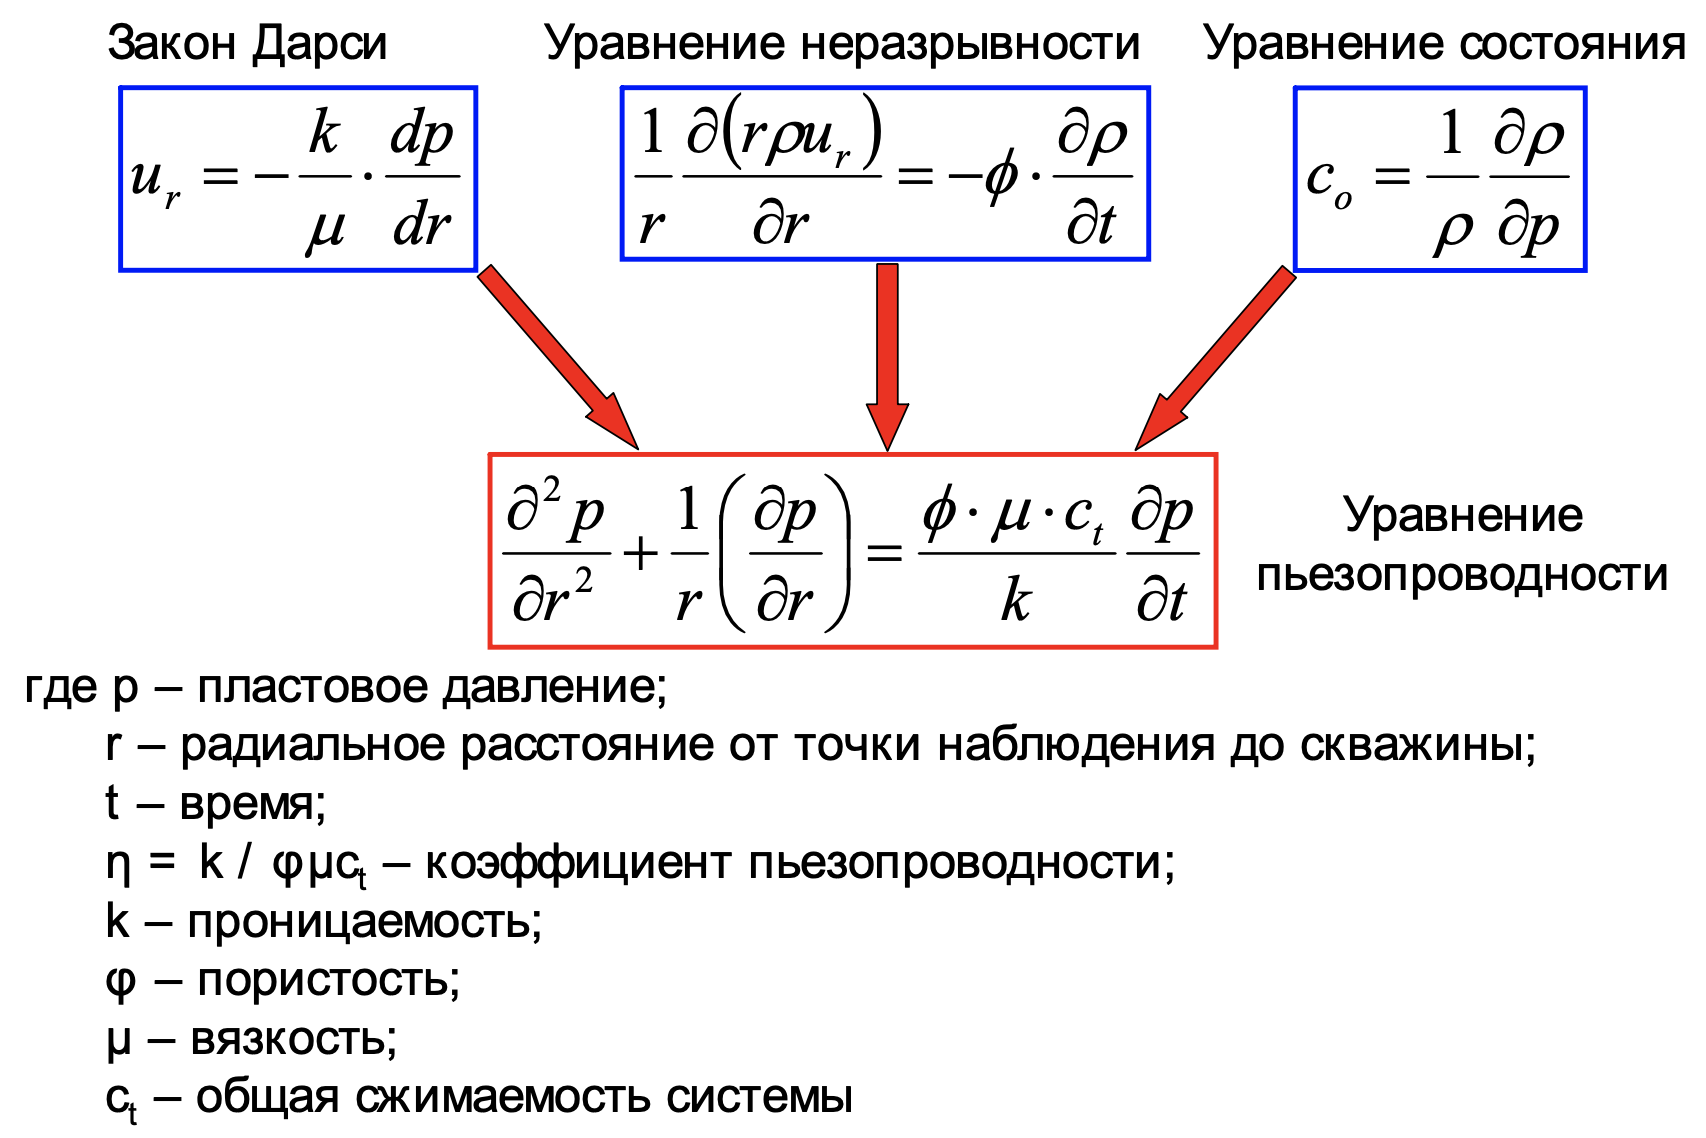
\includegraphics[width=\textwidth]{get_piezoconductivity}

Уравнение пьезопроводности -- основное уравнение для моделирования фильтрации потока.
\\

Коэффициент пьезопроводности пласта -- коэффициент, характеризующий темпы распределения пластового давления в условиях упругого режима, равный отношению коэффициента проницаемости пласта к произведению вязкости жидкости на коэффициент упругости.

\end{document}